\section{Structure du projet}

\textbf{NB:}
La grande majorité de notre application a été réalisée à partir des librairies officielles Android. Nous avons nous mêmes implémenté nos effets. Nous avons sinon utilisé les composants graphiques fournis avec AndroidStudio (dont certains à installer, notamment \textbf{RecyclerView}). Enfin nous avons importé le composant \textbf{PhotoView} en plus des composants Android.

\subsection{Structure graphique Android et navigation :}\label{navig}
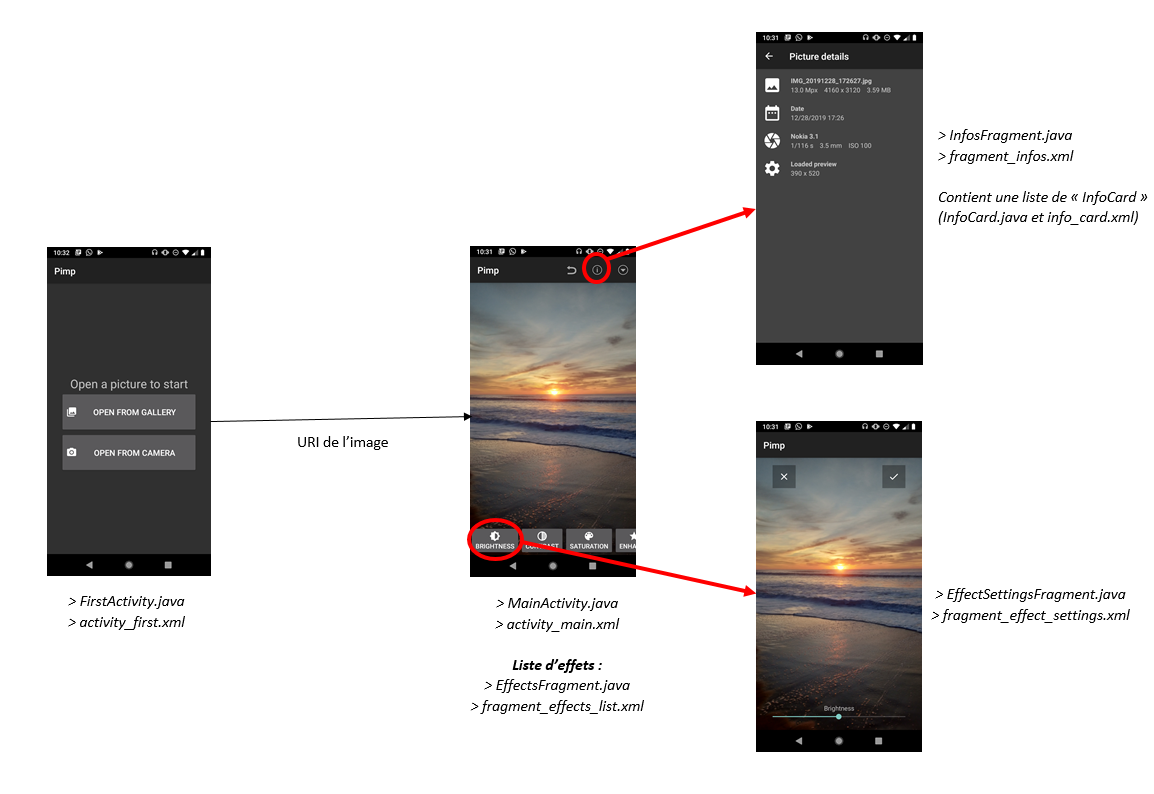
\includegraphics[width=1\textwidth]{report_src/app_flowchart_fragments.PNG}

Pour afficher certains éléments d'interface comme par exemple les informations de l'image (bouton \faInfoCircle) nous utilisons des \textbf{Fragment}. En effet une activité supplémentaire n'est pas nécessaire car cette petite partie de l'application ne correspond pas à un point d'entrée de l'application. Par ailleurs changer de fragment (plutôt que de changer directement de layout) pourrait faciliter l'implémentation d'une interface différente, pour tablette par exemple.
De même, la liste d'effets et leurs paramètres respectifs sont aussi contenus dans des fragments séparés. Cela permet de gérer plus simplement leur affichage et de clarifier le code.
\\

On notera que dans la structure actuelle de l'application, l'image actuellement éditée est contenue et manipulée depuis l'activité principale. Les fragments n'apportent à l'application que des éléments d'interface.
\\

Une seconde activité est cependant utilisée pour la page d'accueil à l'ouverture de l'application, cette \textbf{FirstActivity} utilise des méthodes génériques de \textbf{ActivityIO} afin de gérer l'ouverture de la galerie ou de la caméra. L'application reste dans cette activité tant qu'une \textbf{Uri} valable ($\approx$ chemin) n'a pas été sélectionnée. Ensuite cette Uri est transférée à \textbf{MainActivity} qui va alors charger cette première Image, en cas de problème de chargement l'application peut retourner dans FirstActivity.

\subsection{Classe \textbf{Image}} \label{classeImage}
Cette classe a été conçu comme une alternative à l'utilisation directe de la classe \textbf{Bitmap} fournie par Android.
\\
Le coeur de la classe est évidement une instance de Bitmap, qu'il est possible de récupérer à tout moment. Par ailleurs la classe offre des fonctionnalités supplémentaires, parmi celle ci notamment la possibilité de restaurer l'image à son état au moment de sa création ou de son chargement via la méthode \textbf{reset()}, ou d'annuler les dernières modifications apportées par un effet grâce aux méthodes \textbf{quicksave()} et \textbf{discard()}.
\\

On notera la nécessité pour Image d'avoir la référence d'une Activité de l'application, en effet elle est requise à plusieurs moments par les librairies Android pour charger la Bitmap en mémoire.

\subsubsection{Classe \textbf{ImageInfo}}
La classe Image \ref{classeImage} génère et garde une instance de la classe \textbf{ImageInfo}, cette classe contient un grand nombre de valeurs à propos de l'Image (dimensions, coordonnées GPS, date de prise de vue, ...).
\\
L'idée de cette classe était d'empaqueter toutes ces informations afin de faciliter le passage de ces informations à travers des Fragments ou des Activités (voir \ref{navig}). On notera que tous les accesseurs appliquent des opérations de formatage sur ces données, certaines opérations pourraient être déplacées dans les constructeurs si elles venaient à être utilisées régulièrement.


\subsubsection{File d'effets} \label{file_effets}
Pour pouvoir exporter l'image éditée, il est nécessaire de ré appliquer sur l'image d'origine tout les effets appliqués à l'image affichée dans l'application.
\\
C'est pourquoi la classe Image permet d'empaqueter une file de \textbf{ImageEffect}. Les ImageEffect permettent de transporter des méthodes d'effets, en effet en définissant la méthode \textbf{run()} de l'interface \textbf{ImageEffectCommand} avec une lambda on peut empaqueter un effet applicable à un objet \textbf{Bitmap}. Ce qui permet de passer n'importe quel effet venant de n'importe quel auteur, ce qui renforce la modularité des effets et de la classe Image.
\\
Attention pour correctement utiliser l'historique, il est nécessaire d'appliquer les effets en passant par la classe Image et la méthode \textbf{applyEffect(...)} et non en appelant soi-même un effet et en passant la Bitmap de l'image. (Cela fonctionnera mais l'historique ne sera pas pris en compte et l'export pourrait ne pas marcher)

\subsubsection{Classe ImagePack}
Cette classe un peu particulière fournie dans le package image n'est utile que lors de l'utilisation d'aperçus d'image et avec une utilisation bien précise de \textbf{quickSave()} et \textbf{discard()}. A savoir sauvegarder l'image quand l'on confirme un effet, pour pouvoir la restaurer si un évenxtuel futur effet actif n'est finalement pas choisi par l'utilisateur (bouton annuler).
\\
Ainsi avec cette classe il est possible de regrouper l'image actuellement éditée et une batterie d'aperçus de différents effets. Des méthodes sont à disposition pour faciliter la confirmation d'un effet ou la réinitialisation de l'image d'origine.



\subsection{AsyncTasks}
Les 3 classes du package \textbf{fr.ubordeaux.pimp.task} héritent de la classe Android \textbf{AsyncTask} et permettent d'exécuter certaines opérations en arrière plan, donc sans bloquer l'interface utilisateur.
\\
Ainsi \textbf{LoadImageUriTask} et \textbf{ExportImageTask} permettent respectivement de charger une image et de l'exporter, elles s'occupent d'afficher un petit logo de chargement et de lancer les calculs.
\\
\textbf{ApplyEffectTask} est un peu différente, elle permet de mettre en arrière plan le calcul d'application d'un effet. Elle fonctionne pour n'importe quel effet, pour ce faire elle a besoin d'un paramètre, le type d'effet sous la forme d'un \textbf{ImageEffect}.

\subsection{Classes d'effets}
Les effets applicables dans notre application sur des Bitmap sont rangés dans 3 classes du package \textbf{fr.ubordeaux.pimp.filters}.
\\
\textbf{Retouching} contient les effets les plus classiques d'amélioration d'une image et notamment ceux utilisant des histogrammes (luminosité, contraste, et saturation).
\\
\textbf{Color} contient tout les effets ayant un impact sur la colorimétrie de l'image (modification de teinte, noir et blanc et sélection de couleur).
\\
\textbf{Convolution} contient tout les effets utilisant des méthodes de convolution (flou, détection de contour etc).
\\
\textbf{NB:} Tous nos effets ne sont pas implémentés directement en Java comme le reste du code mais font appel à des scripts RenderScript en C, ce qui accélèrent considérablement l'application des effets.

\subsection{Fragment \textbf{EffectSettingsFragment}} \label{effect_settings}
Ce fragment un peu particulier joue le rôle le plus important dans l'application des effets sur l'image, en effet selon le bouton d'effet sélectionné il génère les curseurs nécessaires au paramétrage de l'effet.
\\
Leur nombre peut varier d'un effet à l'autre mais également leur fourchette de valeurs, ainsi cette classe convertit les méthodes d'effets et leurs arguments en éléments d'interfaces pour l'utilisateur.

\subsection{Packages utilitaires}
De nombreuses classes du code permettent une factorisation et une clarification du code en offrant des méthodes pratiques, généralement statiques. Parmi ces classes on pourra retrouver:
\\

La classe \textbf{Utils} qui offre des méthodes pour récupérer la taille de l'écran, pour calculer un ratio de redimensionnement, pour manipuler des chemins d'image ou régler des problèmes d'orientation d'image.
\\

La classe \textbf{BitmapIO} permet d'effectuer le chargement d'une Bitmap de plusieurs manières, depuis les resources ou un autre emplacement du téléphone, et avec la taille voulue.
\\

La classe \textbf{ActivityIO} permet de gérer l'ouverture de l'application de galerie ou de caméra et d'en récupérer le retour, le tout en gérant les permissions de l'application.
\\

Enfin la classe \textbf{Kernels} offre des méthodes de génération de noyau de convolution permettant de créer différents effets.
\\

\subsection{Modularité du code}
\begin{center}
    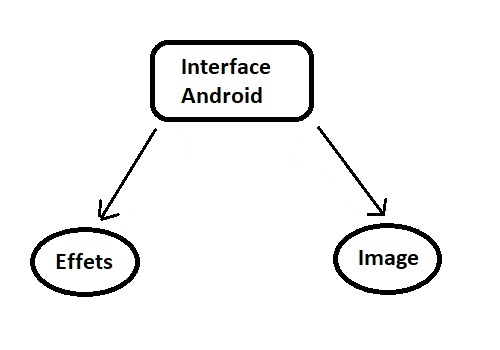
\includegraphics[width=0.7\textwidth]{report_src/structure.jpg}
\end{center}
Notre code a été conçu en 3 grandes parties, la partie principale regroupe toutes les activités, les fragments, les tâches, ... Cette partie utilise des instances de la classe Image, et fait appel à nos méthodes d'effets.
\\

Cette structure permet une grande modularité du code, notre classe Image tout comme nos effets sont facilement exportables pour être utilisés sur un autre projet, on peut imaginer créer une autre application avec les mêmes effets mais une interface complètement différente.
\\
A l'inverse si nous voulions récupérer des effets sur un autre projet il est tout à fait possible de les ajouter au projet, il suffira alors de rajouter en conséquence un bouton dans notre interface et un comportement pour \textbf{EffectSettingsFragment} \ref{effect_settings}
